%% -*- mode: Rnw; coding: utf-8; -*-
%\VignetteIndexEntry{Local polynomial regression in two variables: Estimating partial derivatives}
%\VignetteDepends{Deriv,Ryacas,ggplot2,gridExtra,lattice,stringi,stringr}
%\VignetteKeywords{nonparametric}
%\VignettePackage{interp}

\documentclass[nojss]{jss}
\usepackage[utf8]{inputenc}
%\usepackage{Sweave}
\usepackage{amsfonts}
\usepackage{amssymb}
\usepackage{amsmath}
\usepackage{amsthm}
\usepackage{bm}
\usepackage{graphicx}

% put floats before next section:
\usepackage[section]{placeins}

% collect appendices as subsections
\usepackage[toc,page]{appendix}

% customize verbatim parts
\usepackage{listings}
\lstdefinestyle{Sstyle}{
  basicstyle=\ttfamily\rsize,
  columns=fixed,
  breaklines=true, % sets automatic line breaking
  breakatwhitespace=false,
  postbreak=\raisebox{0ex}[0ex][0ex]{\ensuremath{\color{red}\hookrightarrow\space}},
  fontadjust=true,
  basewidth=0.5em,
  inputencoding=utf8,
  extendedchars=true,
  literate={‘}{{'}}1 {’}{{'}}1 % Zeichencodes für Ausgabe von lm() !
  {á}{{\'a}}1 {é}{{\'e}}1 {í}{{\'i}}1 {ó}{{\'o}}1 {ú}{{\'u}}1
  {Á}{{\'A}}1 {É}{{\'E}}1 {Í}{{\'I}}1 {Ó}{{\'O}}1 {Ú}{{\'U}}1
  {à}{{\`a}}1 {è}{{\`e}}1 {ì}{{\`i}}1 {ò}{{\`o}}1 {ù}{{\`u}}1
  {À}{{\`A}}1 {È}{{\'E}}1 {Ì}{{\`I}}1 {Ò}{{\`O}}1 {Ù}{{\`U}}1
  {ä}{{\"a}}1 {ë}{{\"e}}1 {ï}{{\"i}}1 {ö}{{\"o}}1 {ü}{{\"u}}1
  {Ä}{{\"A}}1 {Ë}{{\"E}}1 {Ï}{{\"I}}1 {Ö}{{\"O}}1 {Ü}{{\"U}}1
  {â}{{\^a}}1 {ê}{{\^e}}1 {î}{{\^i}}1 {ô}{{\^o}}1 {û}{{\^u}}1
  {Â}{{\^A}}1 {Ê}{{\^E}}1 {Î}{{\^I}}1 {Ô}{{\^O}}1 {Û}{{\^U}}1
  {œ}{{\oe}}1 {Œ}{{\OE}}1 {æ}{{\ae}}1 {Æ}{{\AE}}1 {ß}{{\ss}}1
  {ű}{{\H{u}}}1 {Ű}{{\H{U}}}1 {ő}{{\H{o}}}1 {Ő}{{\H{O}}}1
  {ç}{{\c c}}1 {Ç}{{\c C}}1 {ø}{{\o}}1 {å}{{\r a}}1 {Å}{{\r A}}1
  {€}{{\euro}}1 {£}{{\pounds}}1 {«}{{\guillemotleft}}1
  {»}{{\guillemotright}}1 {ñ}{{\~n}}1 {Ñ}{{\~N}}1 {¿}{{?`}}1
}
% switch to above defined style
\lstset{style=Sstyle}

% nice borders for code blocks
\usepackage{tcolorbox}
% enable boxes over several pages:
\tcbuselibrary{breakable,skins}
\tcbset{breakable,enhanced}

\definecolor{grey2}{rgb}{0.6,0.6,0.6}
\definecolor{grey1}{rgb}{0.8,0.8,0.8}



% some abbreviations:
\newcommand{\R}{\mathbb{R}}
\newcommand{\EV}{\mathbb{E}}
\newcommand{\Vect}[1]{\underline{#1}}
\newcommand{\Mat}[1]{\boldsymbol{#1}}
\newcommand{\Var}{\mbox{Var}}
\newcommand{\Cov}{\mbox{Cov}}
% lstinline can break code across lines
\def\cmd{\lstinline[basicstyle=\ttfamily,keywordstyle={},breaklines=true,breakatwhitespace=false]}
% but lstinline generates ugly sectionnames in PDF TOC, so use \texttt there
\newcommand{\cmdtxt}[1]{\texttt{#1}}

\newtheorem{definition}{Definition}[section]
\newtheorem{remark}{Remark}[section]
\newtheorem{lemma}{Lemma}[section]

%%%%%%%%%%%%%%%%%%%%%%%%%%%%%%
%% declarations for jss.cls %%%%%%%%%%%%%%%%%%%%%%%%%%%%%%%%%%%%%%%%%%
%%%%%%%%%%%%%%%%%%%%%%%%%%%%%%

%% almost as usual
\author{
  Albrecht Gebhardt\\ %Department of Statistics,
  University Klagenfurt
\And
  Roger Bivand\\ %Department of Economics,
  Norwegian School of Economics}

\title{Local Polynomial Regression: How the \proglang{R} Package
  \pkg{interp} estimates partial derivatives for later use in Spline
  Interpolation}

%% for pretty printing and a nice hypersummary also set:
\Plainauthor{Albrecht Gebhardt, Roger Bivand} %% comma-separated
\Plaintitle{Local Polynomial Regression: How the R Package interp estimates partial derivatives for later use in Spline Interpolation} %% without formatting
\Shorttitle{Local Polynomial Regression in \proglang{R} Package \pkg{interp}} %% a short title (if necessary)

%% an abstract and keywords
\Abstract{
This vignette presents the \proglang{R} package \pkg{interp}
and focuses on local polynomial regression for estimating partial derivatives.

This is the first of planned three vignettes for this package (not yet finished).
}
\Keywords{local polynomial regression, partial derivatives, \proglang{R} software}
\Plainkeywords{local polynomial regression, partial derivatives, R software}
%% without formatting
%% at least one keyword must be supplied

%% publication information
%% NOTE: Typically, this can be left commented and will be filled out by the technical editor
%% \Volume{13}
%% \Issue{9}
%% \Month{September}
%% \Year{2004}
%% \Submitdate{2004-09-29}
%% \Acceptdate{2004-09-29}

%% The address of (at least) one author should be given
%% in the following format:
\Address{
  Albrecht Gebhardt\
  Institut für Statistik\\
  Universität Klagenfurt\
  9020 Klagenfurt, Austria\\
  E-mail: \email{albrecht.gebhardt@aau.at}\
  %URL: \url{http://statmath.wu-wien.ac.at/~zeileis/}
}
%% It is also possible to add a telephone and fax number
%% before the e-mail in the following format:
%% Telephone: +43/1/31336-5053
%% Fax: +43/1/31336-734

%% for those who use Sweave please include the following line (with % symbols):
%% need no \usepackage{Sweave.sty}

%% end of declarations %%%%%%%%%%%%%%%%%%%%%%%%%%%%%%%%%%%%%%%%%%%%%%%

% for Sinput to set font size of R input code:
\newcommand\rsize{%
   \fontsize{8.5pt}{9.1pt}\selectfont%
}

\begin{document}
% undefine Sinput, Soutput, Scode to be able to redefine them as
% \lstnewenvironment{Sinput}...
\makeatletter
\let\Sinput\@undefined
\let\endSinput\@undefined
\let\Soutput\@undefined
\let\endSoutput\@undefined
\let\Scode\@undefined
\let\endScode\@undefined
\makeatother

\hypersetup{pdftitle={Local Polynomial Regression: How the R Package interp estimates partial derivatives for later use in Spline Interpolation},pdfauthor={Albrecht Gebhardt and Roger Bivand},
  pdfborder=1 1 1 1 1}

% Sweave stuff:
% graphics dimension:
\setkeys{Gin}{width=0.8\textwidth}
%\setkeys{Gin}{width=1in}
% all in- and output black:
\definecolor{Sinput}{rgb}{0,0,0}
\definecolor{Soutput}{rgb}{0,0,0}
\definecolor{Scode}{rgb}{0,0,0}
% redefine Sinput, Soutput, Scode, variant 1 use fancy verbatim
%
%\DefineVerbatimEnvironment{Sinput}{Verbatim}
% gobble=0 !!! otherwise 2 characters of S lines are hidden !!!
%{formatcom = {\color{Sinput}},fontsize=\rsize,xleftmargin=2em,gobble=0}
%\DefineVerbatimEnvironment{Soutput}{Verbatim}
%{formatcom = {\color{Soutput}},fontsize=\rsize,xleftmargin=2em,gobble=0}
%\DefineVerbatimEnvironment{Scode}{Verbatim}
%{formatcom = {\color{Scode}},fontsize=\rsize,xleftmargin=2em,gobble=0}
%\fvset{listparameters={\setlength{\topsep}{0pt}}}
%\renewenvironment{Schunk}{\vspace{\topsep}}{\vspace{\topsep}}
%
% redefine Sinput, Soutput, Scode, variant 2, use color boxes (tcb)
\lstnewenvironment{Sinput}{\lstset{style=Sstyle}}{}%
\lstnewenvironment{Soutput}{\lstset{style=Sstyle}}{}%
\lstnewenvironment{Scode}{\lstset{style=Sstyle}}{}%
\renewenvironment{Schunk}{\vspace{\topsep}\begin{tcolorbox}[breakable,colback=grey1]}{\end{tcolorbox}\vspace{\topsep}}
% see http://www.stat.auckland.ac.nz/~ihaka/downloads/Sweave-customisation.pdf
%

% all in one line!!! setting for direct PDF output !


% Sweave initialization:
% restrict line length of R output, no "+" for continued lines,
% set plot margins:
% initialize libraries and RNG if necessary


\section[Note]{Note}
\label{sec:note}
Notice: This is a preliminary and not yet complete version of this vignette.
Finally three vignettes will be available for this package:
\begin{enumerate}
\item this one related to partial derivatives estimation,
\item a next one describing interpolation related stuff
\item and a third one dealing with triangulations and voronoi mosaics.
\end{enumerate}
Currently only the first text is available and not yet finished.

\section[Introduction]{Introduction}
\label{sec:intro}
Altough the main intention of this \cmd{R} package is
interpolation, it also contains routines for local polynomial
regression. The reason is that the spline interpolation implemented by
\cmd{interp::interp(...,method="akima")} needs estimates of the
partial derivatives of the interpolated function up to degree 2.

One approach to get such estimates is to perform a local polynomial
regression \citep[see e.g.][p. 19]{fan1996local} and get the 
partial derivatives as a side
effect, as explained later. This is also applied in Akimas original
code in a special hardcoded way (using a fixed local bandwidth and a
uniform kernel). Once this routines had been implemented and used
internally in the \cmd{interp::interp(...,method="akima")} it was an
obvious decision to make these routines also available to end users of
package \cmd{"interp"}.

\section{Kernel Functions}
\label{sec:kernel}
In the next section we will use the notion of kernel functions, so
lets start with this definition.

\begin{definition}
A one-dimensional kernel function\index{kernel function} $K(x)$ is
\begin{enumerate}
\item a density function, hence
  \begin{enumerate}
  \item $K(x)\ge 0$
  \item $\int_{\R}K(x)dx=1$
  \end{enumerate}
  Lets denote the associated stochastic variable with $X_{K}$ for
  easier notation, it otherwise carries no meaning.
\item $K$ has the property $\int_{\R}x\cdot K(x)=0$ (i.e. $\EV X_{K}=0$,
  kernel function is centered at zero) and
  
\item $K$ is assumed to be symmtric $K(-x)=K(x)$ and
\item $0<\int_{\R}x^{2}\cdot K(x)dx=\sigma^{2}_{K}<\infty$, i.e.
  $\Var X_{K}$ exists.
  \end{enumerate}
\end{definition}
The kernel functions currently implemented in this library are listed
in table \ref{tab:kernels}.
\begin{table}[htbp]
  \centering
  \begin{tabular}{l|c|l}
    name & function & support of $K$ (outside: $K(x)=0$)\\
    \hline
    gaussian      & $\frac{1}{\sqrt{2\pi}}e^{-\frac{x^{2}}{2}}$ & $x\in\R$\\
    cosine       & $\frac{1}{2}\cos(x)$ &$x\in(-\frac{\pi}{2},\frac{\pi}{2}]$\\
    epanechnikov & $\frac{3}{4}(1-x^{2})$&$x\in(-1,1]$\\
    biweight     & $\frac{15}{16}(1-x^{2})^{2}$&$x\in(-1,1]$\\
    tricube      & $\frac{70}{81}(1-|x|^{3})^{3}$ &$x\in(-1,1]$\\
    triweight    & $\frac{35}{32}(1-x^{2})^{3}$  &$x\in(-1,1]$\\
    uniform      & $\frac{1}{2}$ & $x\in(-1,1]$\\
    triangular   & $1-|x|$  &$x\in(-1,1]$
  \end{tabular}
\index{kernel functions}
  \caption{kernels}
  \label{tab:kernels}
\end{table}

A common approach to create twodimensional kernel functions is to
derive them from onedimensional kernels as bivariate densities with
independent components:
\begin{eqnarray*}
  K_{X,Y}(x,y)&=&K_{X}(x)K_{Y}(y)
\end{eqnarray*}
Both $K_X$ and $K_Y$ are choosen from the same kernel function type.


\section{Bivariate Local Polynomial Regression}
\label{sec:local-polyn-regr}
Lets start with a data set $\{(\Vect{x}_{i},z_{i})|i=1,\ldots,n\}$
with vectors $\Vect{x}_{i}=(x_{i},y_{i})^{\top}\in\R^{2}$ and real
numbers $z_{i}\in\R$. Assume a trend model
$$
z=m(\Vect{x})+\varepsilon
$$
with independent random errors $\varepsilon$
and a bivariate polynomial of degree $r$ as setup for $m$:
$$
m(\Vect{x})=m(x,y)=\sum_{i=0}^{r}\sum_{j=0}^{r-i}\beta_{ij}x^{i}y^{j}.
$$
Note that the sum of exponents $i$ and $j$ in each term of the sum is
bounded above by $r$.

Local regression aims to minimize a weighted sum of squares where the
weights are determined by a bivariate kernel function centered at the
actual location for prediction $\Vect{x}$ which decreases with increasing
distance from this centering point:
$$
\sum_{k=1}^{n}K_{X}\left(\frac{x-x_k}{h_{x}}\right)K_{Y}\left(\frac{y-y_k}{h_{y}}\right)
\left[z_k-\sum_{i=0}^{r}\sum_{j=0}^{r-i}\beta_{ij}x_k^{i}y_k^{j}\right]^2 \rightarrow Min
$$

A Taylor expansion of $m(x,y)$ in a location
$\Vect{x}_{0}=(x_{0},y_{0})$ can be used as a starting point to
interpret the estimated parameters:
\begin{eqnarray*}
  m(x,y) &=& \sum_{i=0}^{r-1}\sum_{j=0}^{r-1-i}  \frac{\frac{\partial^{i+j} m}{\partial x^{i}\partial y^{j}}(x_0)}{i!j!}(x-x_0)^{i}(y-y_0)^{j}\\
  &=& \sum_{i=1}^{r}\sum_{j=1}^{r-i} \underbrace{\frac{\frac{\partial^{i+j} m}{\partial x^{i-1}\partial y^{j-1}}(x_0)}{(i-1)!(j-1)!}}_{=\beta_{ij}}(x-x_0)^{i-1}(y-y_0)^{j-1}\\
  &=& \sum_{i=1}^{r}\sum_{j=1}^{r-i} \beta_{ij} (x-x_0)^{i-1}(y-y_0)^{j-1}\\
\end{eqnarray*}
With the estimates
$\widehat{\beta}_{ij}, i=1,\ldots,r, j=1,\ldots,r-i$ for a given
location $\Vect{x}$ we evaluate this Taylor expansion at
$\Vect{x}=\Vect{x}_0$, which means that all terms
$(x-x_0)^{i}(y-y_0)^{j}$ with $i>0$ or $j>0$ vanish.  Only the
estimated function and its derivatives at location $\Vect{x}=\Vect{x}_0$ remain:
\begin{eqnarray}
  \label{eq:estderivs}
  \widehat{m}(x,y)&=&\sum_{i=1}^{r}\sum_{j=1}^{r-i}\widehat{\beta}_{ij} (x-x_0)^{i-1}(y-y_0)^{j-1}\\
  &=&\widehat{\beta}_{1,1}y
\end{eqnarray}
The remaining components of $\widehat{\beta}$ can  now be used to estimate
the values of the derivatives of $m$ in
\begin{eqnarray}
  \label{eq:estderiv}
  \widehat{\frac{\partial^{i+j} m}{\partial x^{i}\partial y^{j}}(x_0)}&=&(i-1)!(j-1)!\widehat{\beta}_{ij}, 
                                                              \quad i=1,\ldots,r, j=1,\ldots,r-i
\end{eqnarray}

%FIXME: correct index shifting of $i$ and $j$

\section{Implementation details}
\label{sec:impl}
Function \cmd{interp::locpoly()} returns estimated values of the
regression function as well as estimated partial derivatives up to
order 3 (Akima splines only need derivatives up to order 2). 
This access to the partial derivatives was the main intent
for writing this code as there are already many other local polynomial
regression implementations in R. Beside the univariate local
estimators \cmd{stats::ksmooth()}, \cmd{locpol::locPolSmootherC()} and
\cmd{KernSmooth::locpoly()} (the last two also return univariate
derivatives) the packages \cmd{locfit} and \cmd{sm} provide amongst
other things bivariate local regression methods. But to our knowledge
currently (spring 2022) no bivariate local regression estimators for
partial derivatives exists. 
%(TODO: double check). 
But anyhow, to be
used from within the C++ implementation of \cmd{interp::interp()} we
had to implement this estimator directly also in C++ in package {interp}.


This is a short overview (to be extend in a later version of this document) 
of the steps that had to be implemented:
\begin{itemize}
\item Formulate the normal equations for the above weighted least squares 
problem. 
\item Use package \cmd{RcppEigen} to perform the numeric solution. 
\item Package \cmd{RcppEigen} provides a sample implementaion \cmd{fastLm} to 
solve ordinary (unweighted) least squares problems. We just used this and 
extended it for the weighted case.  
\item \cmd{fastLm} has the option to use different solvers provided 
in \cmd{RcppEigen}. Our implementation inherits these options.
\end{itemize}


\section[Regular Grid]{Application To A Regular Grid}
\label{sec:regular}

We will test \texttt{locpoly()} now with a bicubic polynomial on the
unit square on a \texttt{ng} by \texttt{ng} grid. Later tests using
Franke functions will follow.

Set the $x$ - $y$ size of a square data grid to
\begin{Schunk}
\begin{Sinput}
> ng <- 11
\end{Sinput}
\end{Schunk}
resulting in 121 grid points.

First let us choose a kernel
\begin{Schunk}
\begin{Sinput}
> knl <- "gaussian"
\end{Sinput}
\end{Schunk}
Other Options would have been \texttt{"uniform"}, \texttt{"cosine"},
\texttt{"biweight"}, \texttt{"triweight"}, \texttt{"tricube"} and
\texttt{"epanechikov"}, compare section \ref{sec:kernels}.

Next both a fixed global and a varying local bandwidth is needed:
\begin{Schunk}
\begin{Sinput}
> bwg <- 0.33  
> bwl <- 0.11  
\end{Sinput}
\end{Schunk}
The global bandwidth (=0.33) is interpreted as ratio of the
$x$ and $y$ range respective. So in this example the ``moving window''
of the kernel function covers a rectangular data region of
$1/3\times 1/3=1/9$ of the bounding box of the data set.

The local bandwidth indicates the proportion of the data set choosen
as local search neighbourhood. Its value 0.11 has been choosen
to match the coverage of the global bandwidth above.

Now set the degree of the local polynomial model (maximum supported
value is 3)
\begin{Schunk}
\begin{Sinput}
> dg=3
\end{Sinput}
\end{Schunk}
and define a bicubic polynomial:
\begin{Schunk}
\begin{Sinput}
> f <- function(x,y) (x-0.5)*(x-0.2)*(y-0.6)*y*(x-1)
\end{Sinput}
\end{Schunk}
Now we prepare symbolic derivatives of $f$ both for calculating exact
values (via package \texttt{Deriv}) and for pretty printing (using
package \texttt{Ryacas}). The helper functions used for these
preparation steps are shown in appendix~\ref{sec:appendix}:
\begin{Schunk}
\begin{Sinput}
> df <- derivs(f,dg)
\end{Sinput}
\end{Schunk}
Now build and fill the grid with the theoretical values:
\begin{Schunk}
\begin{Sinput}
> xg <- seq(0,1,length=ng)
> yg <- seq(0,1,length=ng)
> xyg <- expand.grid(xg,yg)
\end{Sinput}
\end{Schunk}
and prepare a finer grid for detailed plotting at a larger
resolution by increasing the grid density by factor 4 in both axes:
\begin{Schunk}
\begin{Sinput}
> af <- 4
> xfg <- seq(0,1,length=af*ng)
> yfg <- seq(0,1,length=af*ng)
> xyfg <- expand.grid(xfg,yfg)
\end{Sinput}
\end{Schunk}
Create coordinate matrices \texttt{xx} and \texttt{yy} as  matching the grid matrix \texttt{fg}
\begin{Schunk}
\begin{Sinput}
> nx <- length(xg)
> ny <- length(yg)
> xx <- t(matrix(rep(xg,ny),nx,ny))
> yy <- matrix(rep(yg,nx),ny,nx)
\end{Sinput}
\end{Schunk}
Now fill all exact results deriven from symbolic computation into the
grid matrices, again one of the helper functions from appendix
\ref{sec:appendix} is used:
\begin{Schunk}
\begin{Sinput}
> ## data for local regression
> fg   <- outer(xg,yg,f)
> ## data for exact plots on fine grid
> ffg <- fgrid(f,xfg,yfg,dg)
\end{Sinput}
\end{Schunk}
Now perform the local regression estimation, get both global and local
bandwidth results:
\begin{Schunk}
\begin{Sinput}
> ## global bandwidth:
> pdg <- interp::locpoly(xg,yg,fg, input="grid", pd="all", h=c(bwg,bwg), solver="QR", degree=dg,kernel=knl,nx=af*ng,ny=af*ng)
> ## local bandwidth:
> pdl <- interp::locpoly(xg,yg,fg, input="grid", pd="all", h=bwl, solver="QR", degree=dg,kernel=knl,nx=af*ng,ny=af*ng)
\end{Sinput}
\end{Schunk}
Now finally generate the plots. Again a collection of helper function
is used here to fit all 10 plots and descriptions in a single plot.
For interested users they are shown in the appendix.
\begin{Schunk}
\begin{Sinput}
> pf <- gg1image2contours(xfg,yfg,ffg$f,pdg$z,pdl$z,xyg,"f")
> pfx <- gg1image2contours(xfg,yfg,ffg$fx,pdg$zx,pdl$zx,xyg,"f_x")
> pfy <- gg1image2contours(xfg,yfg,ffg$fy,pdg$zy,pdl$zy,xyg,"f_x")
> pfxx <- gg1image2contours(xfg,yfg,ffg$fxx,pdg$zxx,pdl$zxx,xyg,"f_xx")
> pfxy <- gg1image2contours(xfg,yfg,ffg$fxy,pdg$zxy,pdl$zxy,xyg,"f_xy")
> pfyy <- gg1image2contours(xfg,yfg,ffg$fyy,pdg$zyy,pdl$zyy,xyg,"f_yy")
> pfxxx <- gg1image2contours(xfg,yfg,ffg$fxxx,pdg$zxxx,pdl$zxxx,xyg,"f_xxx")
> pfxxy <- gg1image2contours(xfg,yfg,ffg$fxxy,pdg$zxxy,pdl$zxxy,xyg,"f_xxy")
> pfxyy <- gg1image2contours(xfg,yfg,ffg$fxyy,pdg$zxyy,pdl$zxyy,xyg,"f_xyy")
> pfyyy <- gg1image2contours(xfg,yfg,ffg$fyyy,pdg$zyyy,pdl$zyyy,xyg,"f_yyy")
> ## t1 and t3 contain pure texts generated hidden in this Sweave file.
> ## t2 contains aas much of the symbolic computation output as possible:
> t2 <- print_f(f,df,3)
\end{Sinput}
\end{Schunk}
Now we use features of the gridExtra package to arrange all texts and plots:
\begin{Schunk}
\begin{Sinput}
> lay<-rbind(c( 1, 2, 3, 3),
            c( 4, 5, 3, 3),
            c( 6, 7, 8, 9),
            c(10,11,12,13))
> gg <- grid.arrange(grobs=gList(ggplotGrob(pf),t1,t2,ggplotGrob(pfx),ggplotGrob(pfy),ggplotGrob(pfxx),ggplotGrob(pfxy),ggplotGrob(pfyy),t3,ggplotGrob(pfxxx),ggplotGrob(pfxxy),ggplotGrob(pfxyy),ggplotGrob(pfyyy)),layout_matrix = lay)
\end{Sinput}
\end{Schunk}
For the resulting plot see figure \ref{fig:poly}. They show a colored background image
with two (a dashed green and a dotted blue) overlay of isolines.
The colored background represents the exact function resp. its exact derivatives.
Dashed green isolines are global bandwidth estimators, dotted blue isolines are local 
nearest neighbour estimates. All three overlays (colors and isolines) share the same 
step sizes for binning the colors and isoline levels.

Due to the nature of the different used functions only a varying part of 
the symbolic derivatives can be shown as text in the picture.


\begin{figure}[htb]
\centering
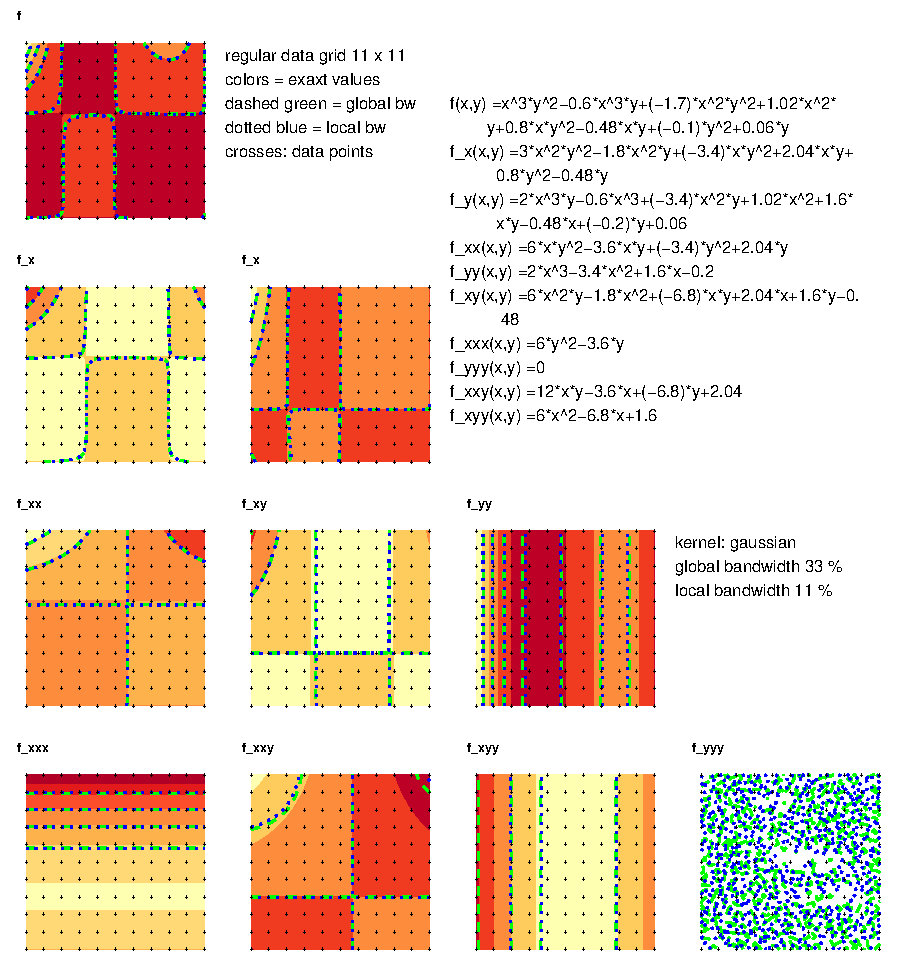
\includegraphics{fig--024}
\caption{A bicubic polynomial and its derivatives, exact and estimated values, regular grid}
\label{fig:poly}
\end{figure}


Now the same steps are repeated for Franke function 1:
\begin{Schunk}
\begin{Sinput}
> f <- function(x,y) 0.75*exp(-((9*x-2)^2+(9*y-2)^2)/4)+0.75*exp(-((9*x+1)^2)/49-(9*y+1)/10)+0.5*exp(-((9*x-7)^2+(9*y-3)^2)/4)-0.2*exp(-(9*x-4)^2-(9*y-7)^2)
> fg  <- outer(xg,yg,f)
> ffg <- fgrid(f,xfg,yfg,dg)
> df  <- derivs(f,dg)
\end{Sinput}
\end{Schunk}
Again estimate with global and local bandwidth
\begin{Schunk}
\begin{Sinput}
> ## global bw,
> pdg <- interp::locpoly(xg,yg,fg, input="grid", pd="all", h=c(bwg,bwg), solver="QR", degree=dg,kernel=knl,nx=af*ng,ny=af*ng)
> ## local bw:
> pdl <- interp::locpoly(xg,yg,fg, input="grid", pd="all", h=bwl, solver="QR", degree=dg,kernel=knl,nx=af*ng,ny=af*ng)
\end{Sinput}
\end{Schunk}
and repeat the plot. Technical details are now hidden and only the
plot is shown as the commands above are more or less repeated.
Results are shown in figure \ref{fig:franke1}. The same interpretation for colors and isolines as in the first plot is applied.
\begin{figure}[htb]
\centering
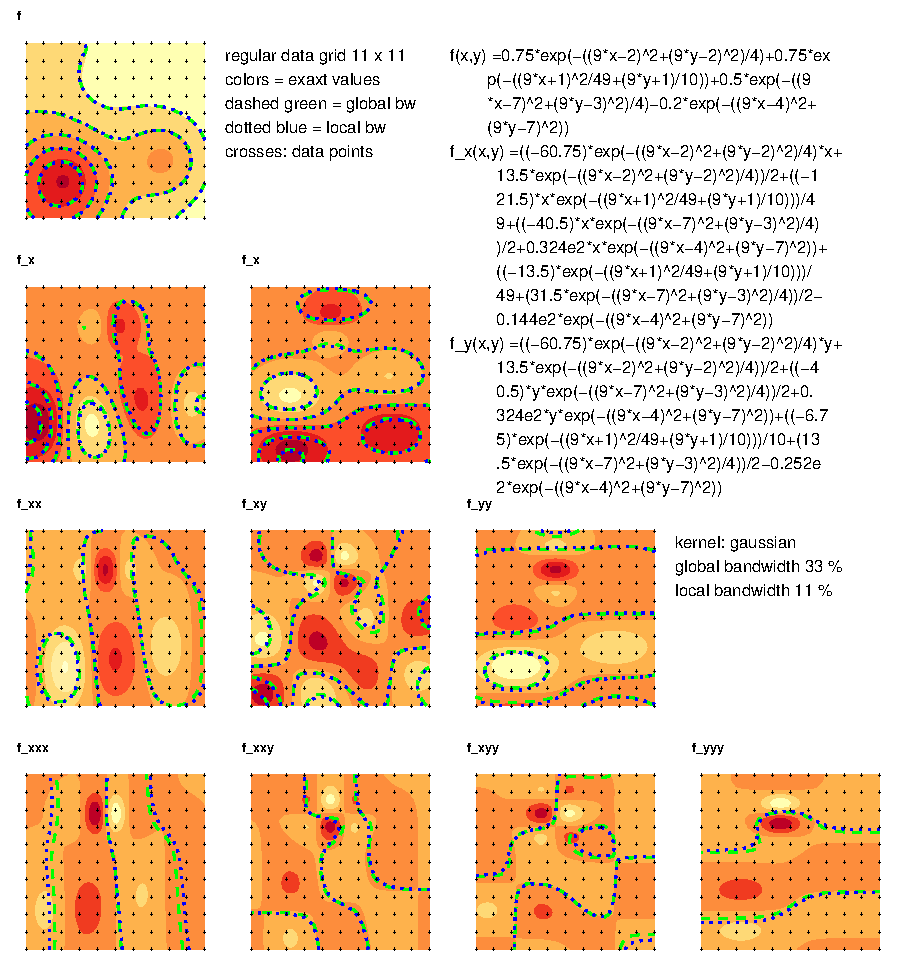
\includegraphics{fig--028}
\caption{Franke function 1 and its derivatives, exact and estimated values, regular grid}
\label{fig:franke1}
\end{figure}


\section[Irregular Grid]{Application To An Irregular Grid}
\label{sec:irreg}

Next we repeat the estmations with an irregular gridded data set using the
same number of $11\times11$=121 points:
\begin{Schunk}
\begin{Sinput}
> n <- ng*ng
\end{Sinput}
\end{Schunk}
Start with the same polynomial as in the last section:
\begin{Schunk}
\begin{Sinput}
> f <- function(x,y) (x-0.5)*(x-0.2)*(y-0.6)*y*(x-1)
\end{Sinput}
\end{Schunk}
The kernel settings stay the same (\cmd{kernel=}"gaussian", global/local bandwidth 0.33/0.11).
\begin{Schunk}
\begin{Sinput}
> ## random irregular data
> x<-runif(n)
> y<-runif(n)
> xy<-data.frame(Var1=x,Var2=y)
> z <- f(x,y)
\end{Sinput}
\end{Schunk}
Again fill the grids for plotting the exact values  
\begin{Schunk}
\begin{Sinput}
> ffg <- fgrid(f,xfg,yfg,dg)
> df <- derivs(f,dg)
\end{Sinput}
\end{Schunk}
and perform the estmation steps:
\begin{Schunk}
\begin{Sinput}
> ## global bandwidth
> pdg <- interp::locpoly(x,y,z, xfg,yfg, pd="all", h=c(bwg,bwg), solver="QR", degree=dg,kernel=knl)
> ## local bandwidth:
> pdl <- interp::locpoly(x,y,z, xfg,yfg, pd="all", h=bwl, solver="QR", degree=dg,kernel=knl)
\end{Sinput}
\end{Schunk}
The remaining steps to generate the plots are again similar to the
first plot and therefore hidden. The output for the bicubic polynomial is shown in figure
\ref{fig:poly2}, results for Franke function 1 in figure \ref{fig:franke12}.
\begin{figure}[htb]
\centering
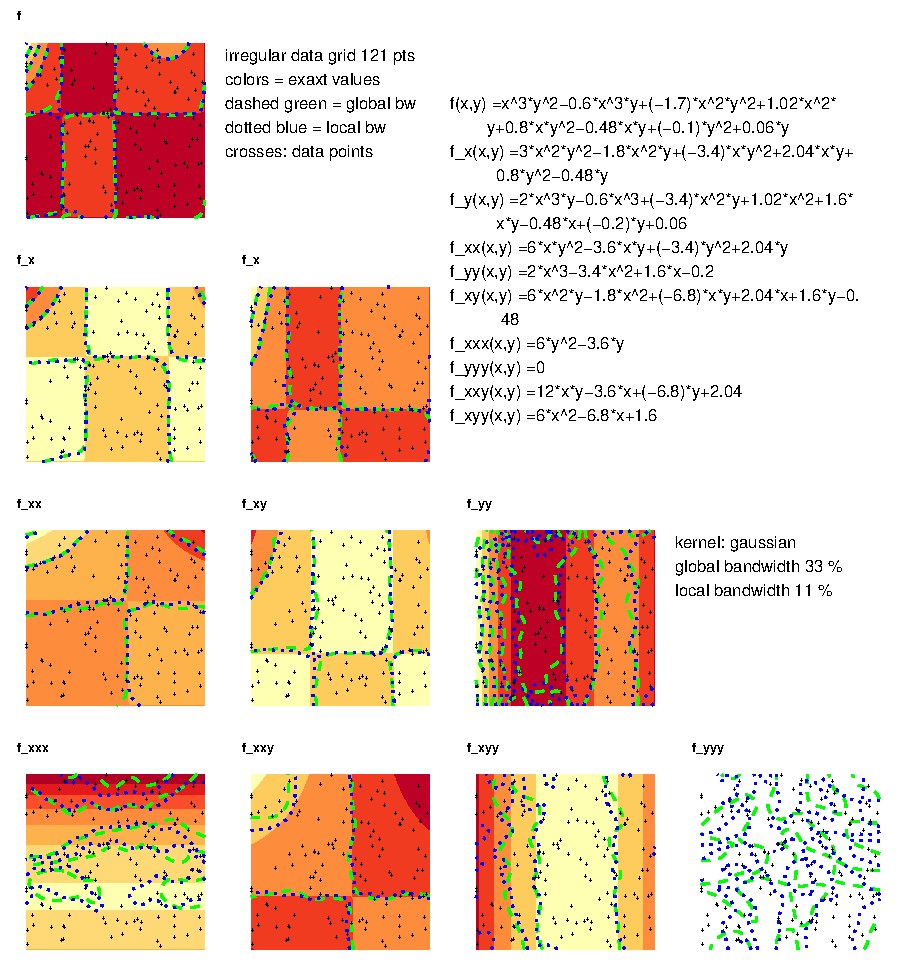
\includegraphics{fig--036}
\caption{A bicubic polynomial and its derivatives, exact and estimated, irregular data set}
\label{fig:poly2}
\end{figure}
The results for Franke function 1 are shown in figure \ref{fig:franke12}. 
\begin{figure}[htb]
\centering
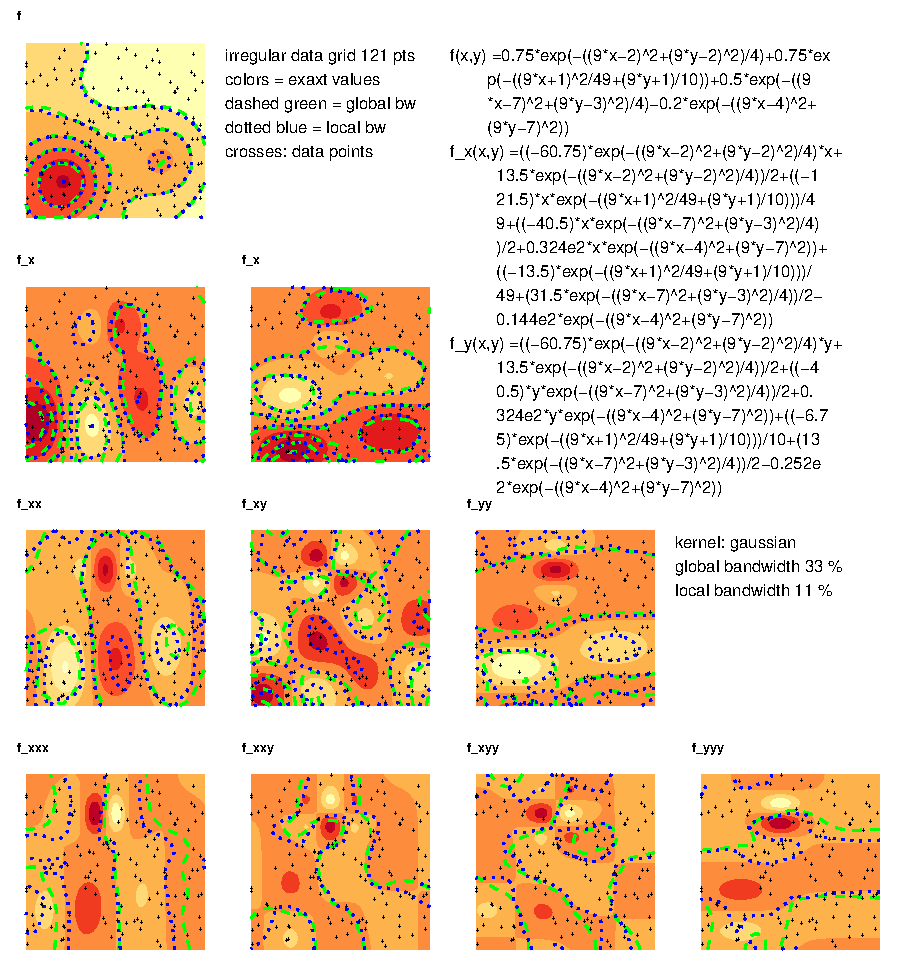
\includegraphics{fig--042}
\caption{Franke function 1 and its derivatives, exact and estimated, irregular data set}
\label{fig:franke12}
\end{figure}

\section{Different Kernels}
\label{sec:kernels}
Now we try different kernels. We just continue with Franke function 1 and
the irregular gridded data from last section. We show the results of \cmd{kernel="uniform"} and 
\cmd{kernel="epanechnikov"} in figures \ref{fig:franke12unif} and \ref{fig:franke12epa}.
\begin{Schunk}
\begin{Sinput}
> ## global bandwidth:
> pdg <- interp::locpoly(x,y,z, xfg,yfg, pd="all", h=c(bwg,bwg), solver="QR", degree=dg,kernel="uniform")
> ## local bandwidth:
> pdl <- interp::locpoly(x,y,z, xfg,yfg, pd="all", h=bwl, solver="QR", degree=dg,kernel="uniform")
\end{Sinput}
\end{Schunk}
\begin{figure}[htb]
\centering
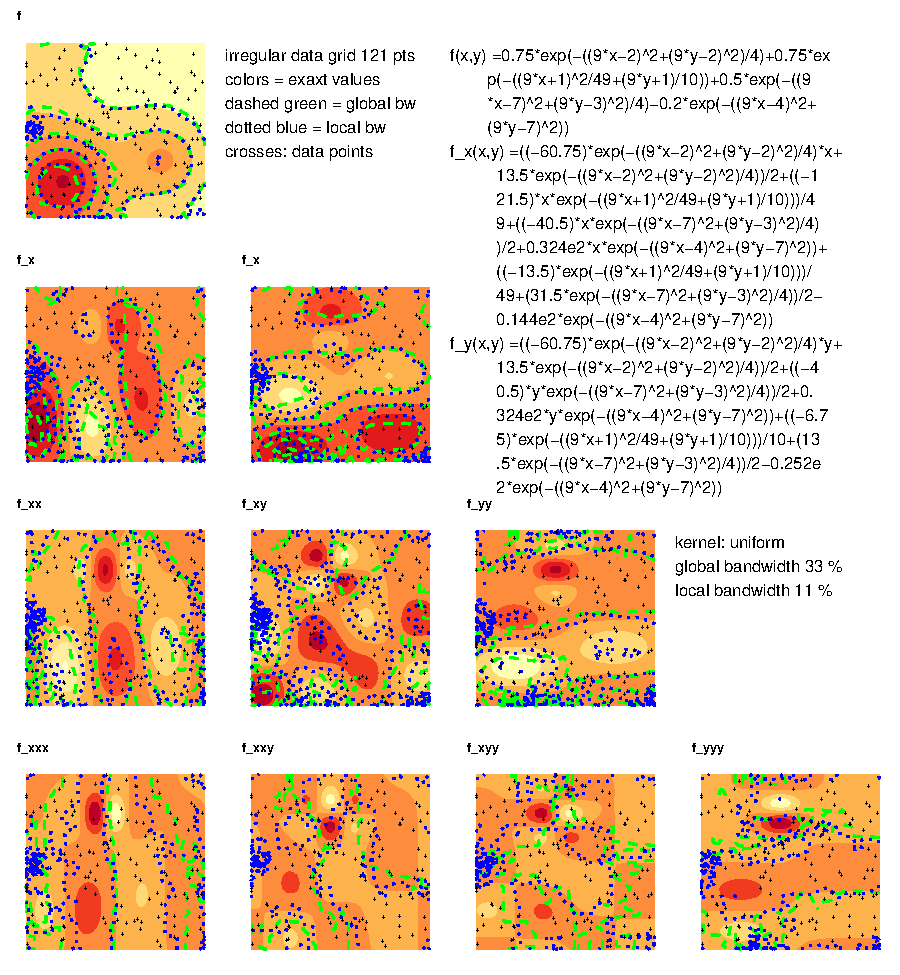
\includegraphics{fig--046}
\caption{Franke function 1 and its derivatives, uniform kernel}
\label{fig:franke12unif}
\end{figure}
\begin{Schunk}
\begin{Sinput}
> ## global bandwidth:
> pdg <- interp::locpoly(x,y,z, xfg,yfg, pd="all", h=c(bwg,bwg), solver="QR", degree=dg,kernel="epanechnikov")
> ## local bandwidth:
> pdl <- interp::locpoly(x,y,z, xfg,yfg, pd="all", h=bwl, solver="QR", degree=dg,kernel="epanechnikov")
\end{Sinput}
\end{Schunk}
\begin{figure}[htb]
\centering
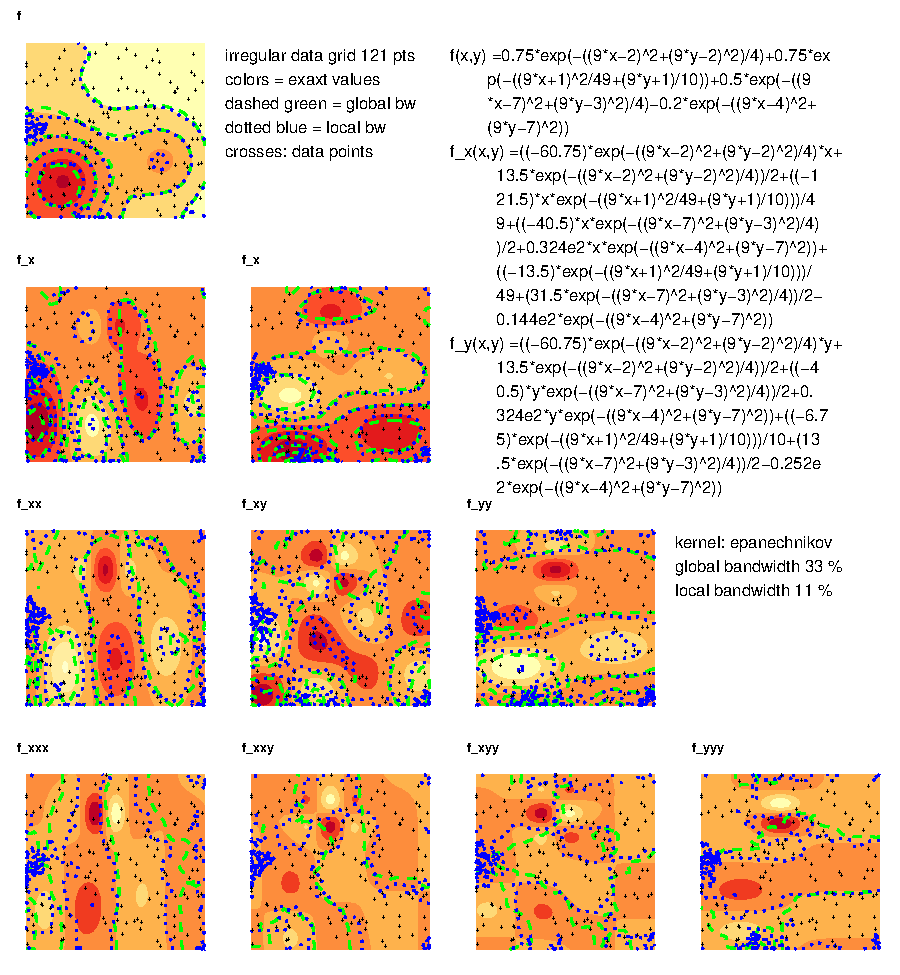
\includegraphics{fig--050}
\caption{Franke function 1 and its derivatives, epanechnikov kernel}
\label{fig:franke12epa}
\end{figure}
Especially the performance of the uniform kernel with its
discontinuous behavior at the borders of its support drops visibly. 
Globally spoken, the local bandwidth estimators capture more details, across all
kernels. But combined with a kernel with bounded support (uniform or
epanechnikov in the test) they show problems at the border of the
region. So the default setting of a gaussian kernel is well founded.
\section{Appendix}
\label{sec:appendix}

These helper functions are needed to convert between \proglang{R}  and  \proglang{Yacas}:
\begin{Schunk}
\begin{Sinput}
> # helper functions for translation between R and Yacas
> fn_y  <- function(f){
     b <- toString(as.expression(body(f)))
     b <- stringr::str_replace_all(b,"cos","Cos")
     b <- stringr::str_replace_all(b,"sin","Sin")
     b <- stringr::str_replace_all(b,"exp","Exp")
     b <- stringr::str_replace_all(b,"log","Log")
     b <- stringr::str_replace_all(b,"sqrt","Sqrt")
     b
 }
> ys_fn  <- function(f){
     f <- stringr::str_replace_all(f,"Cos","cos")
     f <- stringr::str_replace_all(f,"Sin","sin")
     f <- stringr::str_replace_all(f,"Exp","exp")
     f <- stringr::str_replace_all(f,"Log","log")
     f <- stringr::str_replace_all(f,"Sqrt","sqrt")
     f
 }
\end{Sinput}
\end{Schunk}

This function applies symbolic derivatives to a \proglang{R} function,
both for later use as \proglang{R} function (via \pkg{Deriv}) and for
printing (via \pkg{Ryacas}).

\begin{Schunk}
\begin{Sinput}
> derivs <- function(f,dg){
     ret<-list(f=f,
               f_str=ys_fn(yac(paste("Simplify(",y_fn(fn_y(f),""),")"))))
 
     if(dg>0){
 
         ret$fx <- function(x,y){
             myfx <- Deriv(f,"x");
             tmp <- myfx(x,y);
             if(length(tmp)==1)
                 return(rep(tmp,length(x)))
             else
                 return(tmp)
         }
         ret$fx_str  <- ys_fn(yac(paste("Simplify(",y_fn(fn_y(f),"D(x)"),")")))
 
 
         ret$fy <- function(x,y){
             myfy <- Deriv(f,"y");
             tmp <- myfy(x,y);
             if(length(tmp)==1)
                 return(rep(tmp,length(x)))
             else
                 return(tmp)
         }
         ret$fy_str  <- ys_fn(yac(paste("Simplify(",y_fn(fn_y(f),"D(y)"),")")))
 
 
         if(dg>1){
             ret$fxy <- function(x,y){
                 myfxy <- Deriv(Deriv(f,"y"),"x");
                 tmp <- myfxy(x,y);
                 if(length(tmp)==1)
                     return(rep(tmp,length(x)))
                 else
                     return(tmp)
             }
             ret$fxy_str  <- ys_fn(yac(paste("Simplify(",y_fn(fn_y(f),"D(x)D(y)"),")")))
 
             ret$fxx <- function(x,y){
                 myfxx <- Deriv(Deriv(f,"x"),"x");
                 tmp <- myfxx(x,y);
                 if(length(tmp)==1)
                     return(rep(tmp,length(x)))
                 else
                     return(tmp)
             }
             ret$fxx_str  <- ys_fn(yac(paste("Simplify(",y_fn(fn_y(f),"D(x)D(x)"),")")))
 
             ret$fyy <- function(x,y){
                 myfyy <- Deriv(Deriv(f,"y"),"y");
                 tmp <- myfyy(x,y);
                 if(length(tmp)==1)
                     return(rep(tmp,length(x)))
                 else
                     return(tmp)
             }
             ret$fyy_str  <- ys_fn(yac(paste("Simplify(",y_fn(fn_y(f),"D(y)D(y)"),")")))
 
             if(dg>2){
                 ret$fxxy <- function(x,y){
                     myfxxy <- Deriv(Deriv(Deriv(f,"y"),"x"),"x");
                     tmp <- myfxxy(x,y);
                     if(length(tmp)==1)
                         return(rep(tmp,length(x)))
                     else
                         return(tmp)
                 }
                 ret$fxxy_str  <- ys_fn(yac(paste("Simplify(",y_fn(fn_y(f),"D(x)D(x)D(y)"),")")))
 
                 ret$fxyy <- function(x,y){
                     myfxyy <- Deriv(Deriv(Deriv(f,"y"),"y"),"x");
                     tmp <- myfxyy(x,y);
                     if(length(tmp)==1)
                         return(rep(tmp,length(x)))
                     else
                         return(tmp)
                 }
                 ret$fxyy_str  <- ys_fn(yac(paste("Simplify(",y_fn(fn_y(f),"D(x)D(y)D(y)"),")")))
 
                 ret$fxxx <- function(x,y){
                     myfxxx <- Deriv(Deriv(Deriv(f,"x"),"x"),"x");
                     tmp <- myfxxx(x,y);
                     if(length(tmp)==1)
                         return(rep(tmp,length(x)))
                     else
                         return(tmp)
                 }
                 ret$fxxx_str  <- ys_fn(yac(paste("Simplify(",y_fn(fn_y(f),"D(x)D(x)D(x)"),")")))
 
                 ret$fyyy <- function(x,y){
                     myfyyy <- Deriv(Deriv(Deriv(f,"y"),"y"),"y");
                     tmp <- myfyyy(x,y);
                     if(length(tmp)==1)
                         return(rep(tmp,length(x)))
                     else
                         return(tmp)
                 }
                 ret$fyyy_str  <- ys_fn(yac(paste("Simplify(",y_fn(fn_y(f),"D(y)D(y)D(y)"),")")))
             }
         }
     }
     ret
 }
\end{Sinput}
\end{Schunk}

The next function calculates exact values of the given function on a
grid and fills it with partial derivatives up to degree \proglang{dg}.

\begin{Schunk}
\begin{Sinput}
> # for plots of exact values
> fgrid <- function(f,xg,yg,dg){
   ret <- list(f=outer(xg,yg,f))
   df <- derivs(f,dg)
   if(dg>0){
     ret$fx  <- outer(xg,yg,df$fx)
     ret$fy  <- outer(xg,yg,df$fy)
     if(dg>1){
       ret$fxy <- outer(xg,yg,df$fxy)
       ret$fxx <- outer(xg,yg,df$fxx)
       ret$fyy <- outer(xg,yg,df$fyy)
       if(dg>2){
         ret$fxxy <- outer(xg,yg,df$fxxy)
         ret$fxyy <- outer(xg,yg,df$fxyy)
         ret$fxxx <- outer(xg,yg,df$fxxx)
         ret$fyyy <- outer(xg,yg,df$fyyy)
       }
     }
   }
   ret
 }
\end{Sinput}
\end{Schunk}

Another helper function for formatting function expressions in the plots:
\begin{Schunk}
\begin{Sinput}
> split_str <- function(txt,l){
   start <- seq(1, nchar(txt), l)
   stop <- seq(l, nchar(txt)+l, l)[1:length(start)]
   substring(txt, start, stop)
 }
\end{Sinput}
\end{Schunk}

The combination of image and contour plots are generated by these functions:
\begin{Schunk}
\begin{Sinput}
> grid2df <- function(x,y,z)
     subset(data.frame(x = rep(x, nrow(z)),
                       y = rep(y, each = ncol(z)),
                       z = as.numeric(z)),
            !is.na(z))
> gg1image2contours <- function(x,y,z1,z2,z3,xyg,ttl=""){
     breaks <- pretty(seq(min(z1,na.rm=T),max(z1,na.rm=T),length=11))
     griddf1 <- grid2df(x,y,z1)
     griddf2 <- grid2df(x,y,z2)
     griddf3 <- grid2df(x,y,z3)
     griddf  <- data.frame(x=griddf1$x,y=griddf1$y,z1=griddf1$z,z2=griddf2$z,z3=griddf3$z)
     ggplot(griddf, aes(x=x, y=y, z = z1)) +
         ggtitle(ttl) +
         theme(plot.title = element_text(size = 6, face = "bold"),
               axis.line=element_blank(),axis.text.x=element_blank(),
               axis.text.y=element_blank(),axis.ticks=element_blank(),
               axis.title.x=element_blank(),
               axis.title.y=element_blank(),legend.position="none",
               panel.background=element_blank(),panel.border=element_blank(),panel.grid.major=element_blank(),
               panel.grid.minor=element_blank(),plot.background=element_blank()) +
         geom_contour_filled(breaks=breaks) +
         scale_fill_brewer(palette = "YlOrRd") +
         geom_contour(aes(z=z2),breaks=breaks,color="green",lty="dashed",lwd=0.5) +
         geom_contour(aes(z=z3),breaks=breaks,color="blue",lty="dotted",lwd=0.5) +
         theme(legend.position="none") +
         geom_point(data=xyg, aes(x=Var1,y=Var2), inherit.aes = FALSE,size=1,pch="+")
 }
\end{Sinput}
\end{Schunk}

The expressions for the functions and their derivatives are printed via:
\begin{Schunk}
\begin{Sinput}
> print_deriv <- function(txt,l,at=42){
     ret<-""
     for(t in txt){
         if(stringi::stri_length(t)<at)
             btxt <- t
         else
             btxt <- split_str(t,at)
         ftxt <- rep(paste(rep(" ",stringi::stri_length(l)),sep="",collapse=""),length(btxt))
         ftxt[1] <- l
         ret <- paste(ret,paste(ftxt,btxt,sep="",collapse = "\n"),sep="",collapse = "\n")
     }
     ret
 }
> print_f <- function(f,df,dg,offset=0.8){
   lns <- c(print_deriv(df$f_str,"f(x,y) ="))
   if(dg>=1)
     lns <- c(lns,
     print_deriv(df$fx_str,"f_x(x,y) ="),
     print_deriv(df$fy_str,"f_y(x,y) ="))
   if(dg>=2)
     lns <- c(lns,
     print_deriv(df$fxx_str,"f_xx(x,y) ="),
     print_deriv(df$fyy_str,"f_yy(x,y) ="),
     print_deriv(df$fxy_str,"f_xy(x,y) ="))
   if(dg>=3)
     lns <- c(lns,
     print_deriv(df$fxxx_str,"f_xxx(x,y) ="),
     print_deriv(df$fyyy_str,"f_yyy(x,y) ="),
     print_deriv(df$fxxy_str,"f_xxy(x,y) ="),
     print_deriv(df$fxyy_str,"f_xyy(x,y) ="))
   txt <- grid.text(paste(lns,
     collapse="\n"),gp=gpar(fontsize=8),
     x=0,y=offset,draw=FALSE,
     just = c("left","top"))
   txt
 }
\end{Sinput}
\end{Schunk}

\bibliography{lit}

\addcontentsline{toc}{section}{Tables}
\listoftables
\addcontentsline{toc}{section}{Figures}
\listoffigures

\end{document}
